\documentclass{article}
%=================================================
% Basics
%=================================================
\usepackage{fixltx2e} % Makes \( \) equation style robust, among other
                      % things. Must be the first package.


% Makes ligatured fonts searchable and copyable in pdf readers
\usepackage{cmap} % Load before fontenc 

% Always include these font encodings in your document 
% unless you have a very good reason.
\usepackage[T1]{fontenc}
\usepackage[utf8]{inputenc}

\usepackage{verbatim}

%=============
% Fonts
%=============

\usepackage{lmodern} % Improved version of computer modern
\usepackage[scale=0.88]{tgheros} % Helvetica clone for sans serif font


\newcommand\hmmax{2} % Default is 3.
\newcommand\bmmax{2} % Default is 4.

\usepackage{bm} % boldmath must be called after the package
\providecommand{\mathbold}[1]{\bm{#1}}

%=============
% AMS Packages and fonts
%=============
\usepackage{amsmath,amsbsy,amsgen,amscd,amsthm,amsfonts,amssymb} 

%=============
% Margins and paper size
%=============
\usepackage[centering,top=1.5in,bottom=1.2in,left=1.4in,right=1.4in]{geometry}
\usepackage{parskip}


%=============
% Section headings
%=============
\usepackage[sf,bf,compact]{titlesec}

%=============
% Tables and lists
%=============
\usepackage{booktabs,longtable,tabu} % Nice tables
\setlength{\tabulinesep}{1mm}
\usepackage[font=small,margin=10pt,labelfont={sf,bf},labelsep={space}]{caption}

%=============
% Code output
%=============
% \usepackage{listings}
% \usepackage{minted}




\usepackage{enumitem}
\setitemize{itemsep=0pt} 
\setenumerate{itemsep=0pt}
\setlist{labelindent=\parindent,%  % Recommended by enumitem package
  font=\sffamily}


%=============
% Hyperlink colors
%=============
\usepackage[usenames,dvipsnames]{xcolor}
\definecolor{steelblue}{HTML}{A1BDC7}
\definecolor{orange}{HTML}{D98C21}
\definecolor{silver}{HTML}{B0ABA8}
\definecolor{rust}{HTML}{B8420F}
\definecolor{seagreen}{HTML}{2E6B69}
\definecolor{joshua}{HTML}{FBDC7F}
\definecolor{darksky}{HTML}{154c79}

\colorlet{steelblue}{silver!30!white}
\colorlet{darkorange}{orange!85!black}
\colorlet{darksilver}{silver!85!black}
\colorlet{darksteelblue}{steelblue!85!black}
\colorlet{darkrust}{rust!85!black}
\colorlet{darkseagreen}{seagreen!85!black}

\usepackage{url}
\usepackage[colorlinks=true]{hyperref}
\hypersetup{linkcolor=darkrust}    
\hypersetup{citecolor=darkseagreen}      
\hypersetup{urlcolor=darksilver}     

%=============
% Microtype
%=============
\usepackage[final]{microtype} 

%=====================
% Header
%=====================
% \usepackage{fancyhdr}
% \usepackage{nopageno} % Gets rid of page number at the bottom
% \fancyhf{} % Clear header style
% \renewcommand{\headrulewidth}{0.5pt} % remove the header rule
% \pagestyle{fancy}
% \fancyhead[LE,RO]{\textsf{\small \thepage}}
% 
% \setlength{\headheight}{14pt}
%=====================
% Fix delimiters
%=====================

% Fixes \left and \right spacing issues. See discussion at
% http://tex.stackexchange.com/questions/2607/spacing-around-left-and-right
\let\originalleft\left
\let\originalright\right
\renewcommand{\left}{\mathopen{}\mathclose\bgroup\originalleft}
\renewcommand{\right}{\aftergroup\egroup\originalright}

%=================================================
% Math macros
%=================================================

%=============
% Generalities
%=============
\usepackage{mathtools}
\mathtoolsset{centercolon}  % Makes := typeset correctly for definitions

%%% Equation numbering
%\numberwithin{equation}{section} 

%%% Annotations
\newcommand{\notate}[1]{\textcolor{red}{\textbf{[#1]}}}

%==============
% Symbols
%==============
\let\oldphi\phi
\let\oldeps\epsilon

\renewcommand{\phi}{\varphi}
\renewcommand{\epsilon}{\varepsilon}
\newcommand{\eps}{\varepsilon}

%==============
% Constants
%==============

% Set constants upright
\newcommand{\cnst}[1]{\mathrm{#1}}  
\newcommand{\econst}{\mathrm{e}}

\newcommand{\zerovct}{\vct{0}} % Zero vector
\newcommand{\Id}{\mathbf{I}} % Identity matrix
\newcommand{\onemtx}{\bm{1}}
\newcommand{\zeromtx}{\bm{0}}

%==============
% Sets
%==============
\providecommand{\mathbbm}{\mathbb} % In case we don't load bbm

% Reals, complex, naturals
\newcommand{\R}{\mathbbm{R}}
\newcommand{\C}{\mathbbm{C}}
\newcommand{\K}{\mathbbm{K}}
\newcommand{\N}{\mathbbm{N}}

%==============
% Probability
%==============
\newcommand{\Prob}{\operatorname{\mathbbm{P}}}
\newcommand{\Expect}{\operatorname{\mathbb{E}}}

%==============
% Vectors and matrices 
%==============
\newcommand{\vct}[1]{\mathbold{#1}}
\newcommand{\mtx}[1]{\mathbold{#1}}

\newcommand{\mrange}{\operatorname{range}}
\newcommand{\mnull}{\operatorname{null}}


\usepackage{graphicx}

\title{HW 1}
\author{Karl Hiner}
\date{\today}

\begin{document}
\maketitle	

\section{Linear Regression}

\subsection{a}

\begin{equation} \label{eq:1}
    \hat{w} = (X^TX)^{-1}X^TY
\end{equation}
\begin{equation} \label{eq:2}
    y_i = w^T x_i + \epsilon_i,
\end{equation}
where $\epsilon_i \sim \mathcal{N}(0, \sigma^2)$, $w \in \R^d$, and $\{X^i, Y^i\}$ is the $i$-th data point, with $1 \leq i \leq m$.

Using the normal equation (Eqn. \ref{eq:1}), and the model (Eqn. \ref{eq:2}), derive the expectation $\mathbb{E}\left[\hat{w}\right]$.
Note that here $X$ is fixed, and only $Y$ is random.
\begin{align*}
    \mathbb{E}\left[\hat{w}\right] &= \mathbb{E}\left[(X^TX)^{-1}X^TY\right]&\text{Eqn. \ref{eq:1}}\\
    &= \mathbb{E}\left[(X^TX)^{-1}X^T\left(Xw + \epsilon\right)\right]&\text{Substitute $Y$}\\
    &= \mathbb{E}\left[(X^TX)^{-1}X^TXw + (X^TX)^{-1}X^T\epsilon\right]&\text{Distribute}\\
    &= \mathbb{E}\left[w + (X^TX)^{-1}X^T\epsilon\right]&\text{Simplify}\\
    &= w + (X^TX)^{-1}X^T\mathbb{E}\left[\epsilon\right]&\text{Linearity of expectation}\\
    &= w&\text{Since $\mathbb{E}\left[\epsilon\right] = 0$}
\end{align*}

\subsection{b}

Similarly, derive the variance $\text{Var}\left[\hat{w}\right]$.
\begin{align*}
    \text{Var}\left[\hat{w}\right] &= \text{Var}\left[(X^TX)^{-1}X^T\left(Xw + \epsilon\right)\right]&\text{Eqn. \ref{eq:1}, Substitute $Y$}\\
    &= \text{Var}\left[(X^TX)^{-1}X^TXw + (X^TX)^{-1}X^T\epsilon\right]&\text{Distribute}\\
    &= \text{Var}\left[w + (X^TX)^{-1}X^T\epsilon\right]&\text{Simplify}\\
    &= \text{Var}\left[(X^TX)^{-1}X^T\epsilon\right]&\text{Since $w$ is constant}\\
    &= (X^TX)^{-1}X^T\text{Var}\left[\epsilon\right]X(X^TX)^{-1}&\text{$\text{Var}[\vct{b}^T\mtx{X}] = \vct{b}^T\text{Var}[\mtx{X}]\vct{b}$}\\
    &= (X^TX)^{-1}X^T(\sigma^2I_m)X(X^TX)^{-1}&\text{$\text{Var}\left[\epsilon\right] \triangleq \sigma^2$}\\
    &= \sigma^2(X^TX)^{-1}X^TX(X^TX)^{-1}&\text{Commute $\sigma^2$}\\
    &= \sigma^2(X^TX)^{-1}&\text{Simplify}\\
\end{align*}

\subsection{c}

Under the white noise assumption above, does $\hat{w}$ follow a Gaussian distribution with mean and variance in (a) and (b), respectively?
Why or why not?

\textbf{Answer:} Yes, $\hat{w}$ follows a Gaussian distribution with mean and variance in (a) and (b), respectively.
This is because $\hat{w}$ is a linear combination of the random variables $\epsilon_i$, which are Gaussian by assumption.
Since $\hat{w}$ is a linear combination of Gaussian random variables, it is itself Gaussian, with $\hat{w} \sim \mathcal{N}(w, \sigma^2(X^TX)^{-1})$.

\subsection{d: Weighted linear regression}
Suppose we keep the independence assumption but remove the same variance assumption.
In other words, data points would be still sampled independently, but now they may have different variance $\sigma_i$.
Thus, the variance (the covariance matrix) of $\epsilon$ would still be diagonal, but with different values:

$$\Sigma = \begin{bmatrix}
    \sigma_1^2 & 0 & \cdots & 0\\
    0 & \sigma_2^2 & \cdots & 0\\
    \vdots & \vdots & \ddots & \vdots\\
    0 & 0 & \cdots & \sigma_m^2
\end{bmatrix}$$

Derive the estimator $\hat{w}$ (similar to the normal equations) for this problem using matrix-vector notations with $\Sigma$.

\textbf{Answer:}

We want to minimize
$$\arg\min_w \sum_{i=1}^{m} \frac{1}{\sigma_i^2}(y_i - w^T x_i)^2.$$
In matrix-vector notation, this is equivalent to
$$\arg\min_w (Y - Xw)^T \Sigma^{-1} (Y - Xw).$$
Taking the derivative with respect to $w$ and setting it to zero:
\begin{align*}
    \frac{\partial}{\partial w}\left((Y - Xw)^T \Sigma^{-1} (Y - Xw)\right) &= 0\\
    \frac{\partial}{\partial w}\left(w^T X^T \Sigma^{-1} X w - 2w^T X^T \Sigma^{-1} Y + Y^T \Sigma^{-1} Y\right) &= 0\\
    -2X^T \Sigma^{-1} Y + 2X^T \Sigma^{-1} Xw &= 0\\
    (X^T \Sigma^{-1} X)w &= X^T \Sigma^{-1} Y
\end{align*}
Thus, the weighted least squares estimator $\hat{w}$ is:
$$\hat{w} = (X^T \Sigma^{-1} X)^{-1} X^T \Sigma^{-1} Y$$

\section{Ridge Regression}

For linear regression, it is often assumed that $y_i = w^Tx_i + \epsilon$, where $w, x \in \R^d$ by absorbing the constant term (bias) in an affine hypothesis into $w$, and $\epsilon \sim \mathcal{N}(0, \sigma^2)$ is a Gaussian random variable.
Given $m$ i.i.d. samples $z_i = (x_i, y_i), 1 \leq i \leq m$, we define $Y = (y_1, \cdots, y_m)^T$ and $X = (x_1, \cdots, x_m)^T$.
Thus, we have $Y \sim \mathcal{N}(Xw, \sigma^2I_m)$.
Show that the ridge regression estimate is the mean of the posterior distribution under a Gaussian prior $w \sim \mathcal{N}(0, \tau^2I).$
Find the explicit relation between the regularization parameter $\lambda$ in the ridge regression estimate of the parameter $w$, and the variances $\sigma^2, \tau^2$.

\textbf{Answer:}

The ridge regression estimate is defined as
\begin{align*}
    \hat{w}^{\text{Ridge}} &\triangleq \arg\min_w \sum_{i=1}^{m} (w^T x_i - y_i)^2 + \lambda \|w\|^2\\
    &= \arg\min_w \|Xw - Y\|^2 + \lambda\|w\|^2.
\end{align*}
Taking the derivative with respect to $w$ and setting it to zero results in the following expression for $\hat{w}^{\text{Ridge}}$ (as derived in class and in the text):
\begin{align*}
    \hat{w}^{\text{Ridge}} &= (X^T X + \lambda I)^{-1} X^T Y
\end{align*}
Now, we'll show that this estimator is also the mean of the posterior distribution of $w$ when we assume a Gaussian prior $w \sim \mathcal{N}(0, \tau^2I)$.

The posterior distribution of $w$ is proportional to the product of the likelihood and the prior:
\begin{align*}
    p(w|Y) &\propto p(Y|w)p(w)\\
    &\propto \exp\left(-\frac{1}{2\sigma^2}\|Y - Xw\|^2\right)\exp\left(-\frac{1}{2\tau^2}\|w - 0\|^2\right)\\
    &= \exp\left(-\frac{1}{2\sigma^2}\|Xw - Y\|^2\right)\exp\left(-\frac{1}{2\tau^2}\|w\|^2\right)
\end{align*}
\emph{(We neglect the normalization constant $P(Y)$ since it does not depend on $w$.
We also neglect both of the Gaussian normalizing factors since they do not affect the location of the mode.)}

We want to find the mean of this posterior distribution.
Since multiplying two Gaussian PDFs results in another Gaussian PDF, the posterior is also Gaussian.
The mean of a Gaussian PDF is also its mode, which is the location of its maximum.
We can find this (single) maximum, $\hat{w}^{\text{Mean}}$, by finding where its derivative with respect to $w$ is equal to zero.
\begin{align*}
    -log(p(w|Y)) &\propto -log\left(\exp\left(-\frac{1}{2\sigma^2}\|Xw - Y\|^2\right)\exp\left(-\frac{1}{2\tau^2}\|w\|^2\right)\right)\\
    &= \frac{1}{2\sigma^2}\|Xw - Y\|^2 + \frac{1}{2\tau^2}\|w\|^2\\
    0 &= \dfrac{\partial}{\partial w}\left(\frac{1}{2\sigma^2}\|Xw - Y\|^2 + \frac{1}{2\tau^2}\|w\|^2\right)\\
    0 &= \frac{1}{\sigma^2}X^T(Xw - Y) + \frac{1}{\tau^2}w\\
    0 &= \frac{1}{\sigma^2}X^TXw - \frac{1}{\sigma^2}X^TY + \frac{1}{\tau^2}w\\
    \hat{w}^{\text{Mean}} &= \frac{1}{\sigma^2}\left(\frac{1}{\sigma^2}X^TX + \frac{1}{\tau^2}I\right)^{-1}X^TY
\end{align*}
Now, we can find the value of \(\lambda\) equates \(\hat{w}^{\text{Mean}}\) and \(\hat{w}^{\text{Ridge}}\):
\begin{align*}
    \hat{w}^{\text{Mean}} &= \hat{w}^{\text{Ridge}}\\
    \frac{1}{\sigma^2}\left(\frac{1}{\sigma^2}X^TX + \frac{1}{\tau^2}I\right)^{-1}X^TY &= (X^T X + \lambda I)^{-1} X^T Y\\
    \left(\frac{1}{\sigma^2}X^TX + \frac{1}{\tau^2}I\right)^{-1}\frac{1}{\sigma^2}&= (X^T X + \lambda I)^{-1}\\
    \frac{1}{\sigma^2} (X^T X + \lambda I)&= \frac{1}{\sigma^2}X^TX + \frac{1}{\tau^2}I\\
    \frac{\lambda}{\sigma^2} I &= \frac{1}{\tau^2}I\\
    \lambda &= \frac{\sigma^2}{\tau^2}
\end{align*}
Thus, $\hat{w}^{\text{Mean}} = \hat{w}^{\text{Ridge}}$ if we set $\lambda = \frac{\sigma^2}{\tau^2}$.

\section{Lasso estimator}

The LASSO regression problem can be shown to be the following optimization problem:
$$\min_{\vct{w} \in \R^d}\sum_{i=1}^m{(\vct{w}^T\vct{x}_i - y_i)^2} \text{ subject to } \|\vct{w}\|_1 \leq \lambda,$$
where $\lambda > 0$ is a regularization parameter.
Here, we develop a stochastic gradient descent (SDG) algorithm for this problem, which is useful when we have $m >> d$, where $d$ is the dimension of the parameter space.

\subsection{a}
Write $\vct{w} = \vct{w}^{+} - \vct{w}^{-}$, where $\vct{w}^{+}, \vct{w}^{-} \geq 0$ are the positive and negative parts of $\vct{w}$ respectively.
Let $w_j$ be the $j$th component of $\vct{w}$.
When $w_j \leq 0$, $w_j^{+} = 0$ and $w_j^{-} = -w_j$.
Similarly, when $w_j \geq 0$, $w_j^{+} = w_j$ and $w_j^{-} = 0$.
Find a quadratic function, $Q$, of $\vct{w}^{+}$ and $\vct{w}^{-}$ such that
$$\min_{\vct{w}^{+},\vct{w}^{-} \geq 0}\sum_{i=1}^m{Q(\vct{w}^{+}, \vct{w}^{-})}$$
is equivalent to the above LASSO problem.
Expain the equivalence.

\textbf{Answer:}

[Mohri et al] show in Eqn. 11.33 that the LASSO problem can be rewritten as
$$\min_{\vct{w}^{+},\vct{w}^{-} \geq 0}\sum_{i=1}^{m}\left((\vct{w}^{+} - \vct{w}^{-})^T\vct{x}_i - y_i\right)^2 + \lambda\sum_{j=1}^d{(w_j^{+} + w_j^{-})}.$$

To see why these two formulations are equivalent, consider some optimal solution $\vct{w} = \vct{w}^{+} - \vct{w}^{-}$.
Observe that if both $w^{+}_j$ and $w^{-}_j$ were greater than zero for some $j$, we could adjust both $w^{+}_j$ and $w^{-}_j$ by $-\delta_j = -\min(w^{+}_j, w^{-}_j) > 0$.

This change would not affect the difference $w^{+}_j - w^{-}_j$, but would reduce the sum $w^{+}_j + w^{-}_j$ by $2\delta_j$, improving the regularization term.
This implies the original solution was not optimal, which is a contradition.
Thus, for any optimal solution $\vct{w}$, either $w^{+}_j = 0$ or $w^{-}_j = 0$ for all $j$, and we can conclude the following quadratic function admits the same solutions as the LASSO problem:
$$Q(\vct{w}^{+}, \vct{w}^{-}) = \left((\vct{w}^{+} - \vct{w}^{-})^T\vct{x}_i - y_i\right)^2 + \lambda\sum_{j=1}^d{(w_j^{+} + w_j^{-})}$$

\subsection{b}
[Mohri et al Ex. 11.10] Derive a stochastic gradient descent algorithm for the quadratic program (with affine constraints) in part (a).

\textbf{Answer:}

In stochastic gradient descent, we randomly choose a training pair $(\vct{x}_i, y_i)$ and compute the gradient with respect to this pair.

Here is our quadratic objective function for a single training pair $(\vct{x}_i, y_i)$:
$$Q(\vct{w}^{+}, \vct{w}^{-}) = \left((\vct{w}^{+} - \vct{w}^{-})^T\vct{x}_i - y_i\right)^2 + \lambda\sum_{j=1}^d{(w_j^{+} + w_j^{-})}$$
$Q$ has two parameters, $\vct{w}^{+}$ and $\vct{w}^{-}$, so we need to compute the partial derivatives with respect to each of these parameters:
\begin{align*}
    \frac{\partial Q}{\partial w^{+}_j} &= \frac{\partial}{\partial w^{+}_j}\left((\vct{w}^{+} - \vct{w}^{-})^T\vct{x}_i - y_i\right)^2 + \frac{\partial}{\partial w^{+}_j}\lambda\sum_{j=1}^d{(w_j^{+} + w_j^{-})}\tag*{Split}\\
    &= \frac{\partial}{\partial w^{+}_j}\left((\vct{w}^{+} - \vct{w}^{-})^T\vct{x}_i - y_i\right)^2 + \lambda \vct{I}_d\tag*{Solve regularization term}\\
    &=2\left((\vct{w}^{+} - \vct{w}^{-})^T\vct{x}_i - y_i\right)\frac{\partial}{\partial w^{+}_j}\left((\vct{w}^{+} - \vct{w}^{-})^T\vct{x}_i - y_i\right) + \lambda\tag*{Chain rule}\\
    &=2\left((\vct{w}^{+} - \vct{w}^{-})^T\vct{x}_i - y_i\right)\frac{\partial}{\partial w^{+}_j}\left((\vct{w}^{+})^T\vct{x}_i - (\vct{w}^{-})^T\vct{x}_i\right) + \lambda\tag*{$y_i$ is constant}\\
    &=2\left((\vct{w}^{+} - \vct{w}^{-})^T\vct{x}_i - y_i\right)\frac{\partial}{\partial w^{+}_j}\left((\vct{w}^{+})^T\vct{x}_i\right) + \lambda\tag*{$(\vct{w}^{-})^T\vct{x}_i$ is constant}\\
    &= 2\left((\vct{w}^{+} - \vct{w}^{-})^T\vct{x}_i - y_i\right)x_{i,j} + \lambda\tag*{Only the $j$th component of $\vct{x}_i$ interacts with $w_j$}
\end{align*}
Similarly, we can derive
$$\frac{\partial Q}{\partial w^{-}_j} = -2\left((\vct{w}^{+} - \vct{w}^{-})^T\vct{x}_i - y_i\right)x_{i,j} + \lambda.$$

Our update also enforce the constraint, $\vct{w}^{+}, \vct{w}^{-} \geq 0$.
Here is the final SGD update rule, where $\mu$ is the learning rate:
$$w^{+}_j \leftarrow \max\left(0, w^{+}_j - \mu\frac{\partial Q}{\partial w^{+}_j}\right), w^{-}_j \leftarrow \max\left(0, w^{-}_j - \mu\frac{\partial Q}{\partial w^{-}_j}\right)$$

\subsection{c}
Suppose $X = [x_1, \cdots, x_m]^T$ is orthonormal and there exists a solution $w$ for $Xw = Y$, where $Y = [y_1, \cdots, y_m]^T$ with no more than $k$ non-zero elements.
Can the SGD algorithm get arbitrarily close to $w$?
Explain why or why not.

Based on the theorem of stable recovery of sparse $w$ from Candes, Romberg, and Tao (2004), if there is a true sparse $w$ with fewer than $S$ entries equal to zero, where $X$ satisfies S-restricted isometry, such that $Xw = Y$, then an estimator subject to $\arg\min_w \|w\|_1$ can exactly recover the true $w$.

Any orthonormal matrix $X$ satisfies S-restricted isometry for any $S$.
Specifically, since an othonormal matrix $X$ preserves the length of all vectors, $\|X\vct{x}\| = \|\vct{x}\|$, then $\delta_S = 0$ for any $S$ in
$$(1 - \delta_S)\|\vct{x}\|^2 \leq \|X\vct{x}\|^2 \leq (1 + \delta_S)\|\vct{x}\|^2.$$
With regard to the ability of SGD to recover this $w$, note that $Q$ is the Lagrangian of the LASSO problem, composed of a quadratic term (with a unique global minimum) and the L1 regularization term required for sparse recovery.
Thus, there exists a choice of regularization parameter $\lambda$, and a sufficiently small learning rate $\mu$, s.t. the SGD algorithm will, with high probability, converge to the global minimum of $Q$, and thus the true $w$.

\section{Logistic Regression}
Logistic regression is named after the log-odds of success (the logit of the probability) defined as below:
$$\ln\left(\frac{P[Y=1|X=x]}{P[Y=0|X=x]}\right),$$
where
$$P[Y=1|X=x] = \frac{\exp(w_0 + w^Tx)}{1 + \exp(w_0 + w^Tx)}.$$

\subsection{a}
Show that log-odds of success is a linear function of $X$.

\begin{align*}
    \ln\left(\frac{P[Y=1|X=x]}{P[Y=0|X=x]}\right) &= \ln\left(\frac{P[Y=1|X=x]}{1 - P[Y=1|X=x]}\right)\tag*{Since $Y$ has two possible values}\\
    &= \ln\left(\frac{\frac{\exp(w_0 + w^Tx)}{1 + \exp(w_0 + w^Tx)}}{1 - \frac{\exp(w_0 + w^Tx)}{1 + \exp(w_0 + w^Tx)}}\right)\tag*{Substitute for $P[Y=1|X=x]$}\\
    &= \ln\left(\exp(w_0 + w^Tx)\right)\tag*{Simplify}\\
    &= w_0 + w^Tx\tag*{$\ln\left(e^x\right) = x$}
\end{align*}
Since vector addition and dot product are both linear functions, $w_0 + w^Tx$ is also a linear function of $X$.

\subsection{b}
Show that the logistic loss $L(z) = \log(1 + \exp(-z))$ is a convex function.

If we show that the second derivative of $L(z)$ is nonnegative for all $z$, then we have shown that $L(z)$ is convex.
$$L'(z) = \frac{-\exp(-z)}{1 + \exp(-z)}$$
$$L''(z) = \frac{\exp(-z)}{(1 + \exp(-z))^2}$$

Since \(L''(z) > 0\) for all \(z\), \(L(z)\) is a convex function.

\section{Programming: Recommendation System}

\emph{Problem Summary:}
A rating by user $u$ on movie $i$ is approximated by

\begin{equation} \label{eq:5}
M_{u,i} \approx \sum_{k=1}^{d}{U_{u,k}V_{i,k}}.
\end{equation}
We want to fit each element of $U$ and $V$ by minimizing squared reconstruction error over all training data points.
That is, the objective function we minimize is given by
\begin{equation} \label{eq:6}
E(U,V) = \sum_{u=1}^n\sum_{i=1}^m{(M_{u,i} - U_uV_v^T)^2} = \sum_{u=1}^n\sum_{i=1}^m{(M_{u,i} - \sum_{k=1}^d{U_{u,k}V_{i,k}})^2},
\end{equation}
where $U_u$ is the $u$th row of $U$ and $V_i$ is the $i$th row of $V$.

We use gradient descent:
\begin{equation} \label{eq:8}
    U_{v,k} \leftarrow U_{v,k} - \mu \frac{\partial E}{\partial U_{v,k}}, \quad V_{j,k} \leftarrow V_{j,k} - \mu \frac{\partial E}{\partial V_{j,k}},
\end{equation}
where $\mu$ is the update rate.

\subsection{a}
Derive the update formula in (\ref{eq:8}) by solving the partial derivatives.

\textbf{Answer:}
\begin{align*}
    \frac{\partial E}{\partial U_{v,k}} &= \frac{\partial}{\partial U_{v,k}}\sum_{u=1}^n\sum_{i=1}^m{(M_{u,i} - \sum_{k'=1}^d{U_{u,k'}V_{i,k'}})^2}\\
    &= \sum_{u=1}^n\sum_{i=1}^m{\frac{\partial}{\partial U_{v,k}}(M_{u,i} - \sum_{k'=1}^d{U_{u,k'}V_{i,k'}})^2}\\
    &= \sum_{u=1}^n\sum_{i=1}^m{2(M_{u,i} - \sum_{k'=1}^d{U_{u,k'}V_{i,k'}})\frac{\partial}{\partial U_{v,k}}(M_{u,i} - \sum_{k'=1}^d{U_{u,k'}V_{i,k'}})}\tag*{\text{Chain rule}}\\
    &= \sum_{u=1}^n\sum_{i=1}^m{2(M_{u,i} - \sum_{k'=1}^d{U_{u,k'}V_{i,k'}})(-\frac{\partial}{\partial U_{v,k}}\sum_{k'=1}^d{U_{u,k'}V_{i,k'}})}\tag*{$\frac{\partial}{\partial U_{v,k}}M_{u,i} = 0$}\\
    &= \sum_{i=1}^m{2(M_{v,i} - \sum_{k'=1}^d{U_{v,k'}V_{i,k'}})(-V_{i,k})}\tag*{$\frac{\partial}{\partial U_{v,k}}U_{u,k'}V_{i,k'} = 0, k' \neq k, u \neq v$}\\
    &= -2\sum_{i=1}^m{(M_{v,i} - \sum_{k'=1}^d{U_{v,k'}V_{i,k'}})V_{i,k}}
\end{align*}
\begin{align*}
    \frac{\partial E}{\partial V_{j,k}} &= \frac{\partial}{\partial V_{j,k}}\sum_{u=1}^n\sum_{i=1}^m{(M_{u,i} - \sum_{k'=1}^d{U_{u,k'}V_{i,k'}})^2}\\
    &= \sum_{u=1}^n\sum_{i=1}^m{2(M_{u,i} - \sum_{k'=1}^d{U_{u,k'}V_{i,k'}})(-\frac{\partial}{\partial V_{j,k}}\sum_{k'=1}^d{U_{u,k'}V_{i,k'}})}\tag*{\text{Same first three steps}}\\
    &= \sum_{u=1}^n{2(M_{u,j} - \sum_{k'=1}^d{U_{u,k'}V_{j,k'}})(-U_{j,k})}\tag*{\text{$\frac{\partial}{\partial V_{j,k}}U_{u,k'}V_{j,k'} = 0, k' \neq k, i \neq j$}}\\
    &= -2\sum_{u=1}^n{(M_{u,j} - \sum_{k'=1}^d{U_{u,k'}V_{j,k'}})U_{j,k}}
\end{align*}

\subsection{b}
Redo part (a) using the regularized objective function below:
$$E(U,V) = \sum_{u=1}^n\sum_{i=1}^m{(M_{u,i} - \sum_{k=1}^d{U_{u,k}V_{i,k}})^2} + \lambda\sum_{u, k}{U_{u,k}^2} + \lambda\sum_{i,k}^m{V_{i,k}^2}$$

\begin{align*}
    \frac{\partial E}{\partial U_{v,k}} &= \frac{\partial}{\partial U_{v,k}}\left(\sum_{u=1}^n\sum_{i=1}^m{(M_{u,i} - \sum_{k'=1}^d{U_{u,k'}V_{i,k'}})^2} + \lambda\sum_{u, k'}{U_{u,k'}^2} + \lambda\sum_{i,k'}^m{V_{i,k'}^2}\right)\\
    &= \frac{\partial}{\partial U_{v,k}}\left(\sum_{u=1}^n\sum_{i=1}^m{(M_{u,i} - \sum_{k'=1}^d{U_{u,k'}V_{i,k'}})^2}\right) + \frac{\partial}{\partial U_{v,k}}\lambda\sum_{u=1}^n\sum_{k'=1}^d{U_{u,k'}^2} + \frac{\partial}{\partial U_{v,k}}\lambda\sum_{i,k'}^m{V_{i,k'}^2}\\
    &= -2\sum_{i=1}^m{(M_{v,i} - \sum_{k'=1}^d{U_{v,k'}V_{i,k'}})V_{i,k}} + 2\lambda U_{v,k}
\end{align*}
\begin{align*}
    \frac{\partial E}{\partial V_{j,k}} &= \frac{\partial}{\partial V_{j,k}}\left(\sum_{u=1}^n\sum_{i=1}^m{(M_{u,i} - \sum_{k'=1}^d{U_{u,k'}V_{i,k'}})^2}\right) + \frac{\partial}{\partial V_{j,k}}\lambda\sum_{u, k'}{U_{u,k'}^2} + \frac{\partial}{\partial V_{j,k}}\lambda\sum_{i=1}^m\sum_{k'=1}^d{V_{i,k'}^2}\\
    &= -2\sum_{u=1}^n{(M_{u,j} - \sum_{k'=1}^d{U_{u,k'}V_{j,k'}})U_{j,k}} + 2\lambda V_{j,k}
\end{align*}

\subsection{5.4 Report}

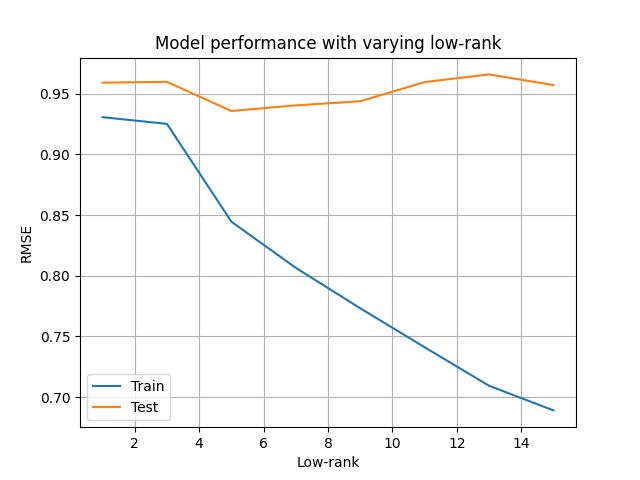
\includegraphics[width=\textwidth]{evaluate}

As shown in the chart above, as \verb|lowRank| increases, the training error decreases monotonically, since the model has more capacity to fit the training data.
However, the error on the test set starts to increase after \verb|lowRank| = 5, indicating that the model is overfitting the training data.
I also found that training for too many iterations resulted in higher test errors, even for small values of \verb|lowRank|.
Thus, using a stopping criteria based on the error, rather than a fixed number of steps across all values of \verb|lowRank|, was important to reduce overfitting.

I used grid search to find the best values of $\mu$ and $\lambda$, using a \verb|lowRank| of 5 and running each iteration to "convergence" (see discussion of error-delta stopping criteria below), or until a maximum number of 1500 gradient descent steps.
I chose to fix the rank at the highest evaluated value of 5 to provide the most degrees of freedom to the model, and thus the most potential for it to (over)fit the data and provide a good signal for evaluating the regularization parameter $\lambda$.
I used the provided train/test split for each run, and did not perform cross-validation.
Here is the relevant code for my hyperparameter search:

\begin{verbatim}
lr = 5 # "Low-rank". Using the highest evaluated value.
max_iter = 1000

best_learn_rate = 0
best_reg_coef = 0
best_rmse = float('inf')
for learn_rate in [0.0001, 0.0002, 0.0004, 0.0005, 0.0008]:
    for reg_coef in [0.001, 0.01, 0.02, 0.04, 0.1, 0.2, 0.4]:
        U, V = run(rate_mat, lr, True, learn_rate, reg_coef, max_iter)
        rmse_val = rmse(U, V, test_mat)
        if rmse_val < best_rmse:
            best_rmse = rmse_val
            best_learn_rate = learn_rate
            best_reg_coef = reg_coef

print('Learn rate: {}, Reg coef: {}'.format(best_learn_rate, best_reg_coef)) 
\end{verbatim}

The best performing values tested for $(\mu, \lambda)$ were $(0.0001, 0.2)$.

My model stop stops gradient descent when the error delta between iterations is less than $10^{-4}$, or when reaching the maximum number of iterations, whichever comes first.
I chose this error delta value empirically by manually searching for values that stop iterating nearly where the validation error (over the provided "test" set) starts to increase for various values of \verb|lowRank|.

\end{document}
